% !TeX spellcheck = it_IT
\newpage
\section{Green coding}
\subsection{Java collections}
Le strutture dati forniscono un modo per organizzare e processare le informazioni. Una struttura \textbf{CRUD} consente di fare quattro operazioni:
\begin{itemize}
	\item \textit{Create}: aggiunta di un elemento
	\item \textit{Read}: lettura di un elemento
	\item \textit{Update}: aggiornamento di un valore
	\item \textit{Delete}: eliminazione di un dato
\end{itemize}
In particolare Java fornisce strutture dati come \textit{List}, \textit{Set} e \textit{Map}. Noi utilizzeremo le prime due. Queste hanno diverse implementazioni con diverse complessità:
\begin{table}[!h]
	\centering
	\begin{tabular}{|c|c|c|c|c|}
		\hline
		\textbf{Struttura} & \textit{Create} & \textit{Read} & \textit{Update} & \textit{Delete} \\
		\hline
		ArrayList & $O(1)$ & $O(1)$ & $O(N)$ & $O(N)$ \\
		LinkedList & $O(N)$ & $O(N)$ & $O(N)$ & $O(N)$\\
		HashSet & $O(1)$ & $O(1)$ & $O(1)$ & $O(1)$\\
		TreeSet & $O(\log N)$ & $O(\log N)$ & $O(\log N)$ & $O(\log N)$\\
		\hline
	\end{tabular}
\end{table}
\begin{note}
	La differenza tra \textit{lista} e \textit{dizionario} è che la prima può contenere duplicati mentre il secondo no.
\end{note}

\subsubsection{Analisi}
Le strutture di tipo \textit{List} sono meno efficienti di quelle \textit{Set}, però possono contenere duplicati. Se si prevede un mix bilanciato di operazioni \textit{ArrayList} è migliore di \textit{LinkedList} tranne per la modifica e l'eliminazione. Alla fine la struttura più efficiente è teoricamente \textit{HashSet}, ma ad esempio se è necessario tenere gli elementi ordinati conviene \textit{TreeSet}.\\
È quindi fondamentale scegliere una struttura dati coerente con il caso di utilizzo.

\subsection{Calcolo approssimato}
Data l'importanza del problema del risparmio energetico, è interessante anche bilanciare all'interno dei linguaggi \textbf{energia} e \textbf{accuratezza}.

\begin{definition}[Calcolo approssimato]
	Il calcolo 	approssimato è una qualunque forma di calcolo il cui risultato non è garantito essere corretto.
\end{definition}
\textbf{EnerJ} estende Java con \textbf{qualificatori di tipo} per dichiarare dati che possono essere approssimati. Il compilatore poi mappa le variabili approssimate su \textbf{memorie a basso voltaggio}, usa \textbf{operazioni a basso consumo} e usa \textbf{algoritmi efficienti}.\\
È dimostrata una riduzione del consumo del $15\%$ in presenza di HW specifico.\\
Il modello di EnerJ è:
\begin{itemize}
	\item \textbf{Sicuro}: il programmatore fa la distinzione tra dati precisi e non, eventualmente forzandolo tramite \textit{endorsement} espliciti
	\item \textbf{Generale}: unifica memoria, calcolo ed operazioni approssimate
\end{itemize}
Tutto questo in un approccio \textbf{"tutto o nulla"} in quanto la precisazione non ha sfumature.

\subsubsection{Annotazioni}
Di default un tipo è \textbf{preciso} e si può quindi omettere
\begin{lstlisting}[language=Java]
	@Precise
\end{lstlisting}
È illegale assegnare una variabile approssimata ad una precisa. Ciò previene un flusso diretto da dati che possono essere approssimati a dati che devono essere precisi.\\
L'unico caso in cui è possibile è tramite \textbf{endorsement}, ovvero un'operazione specificata dal programmatore che \textit{certifica} che questa non produrrà errori sulla parte definita \textit{precisa} nel codice:
\begin{lstlisting}[language=Java]
	@Approx int a = ...;
	int p;
	p = endorse(a);
\end{lstlisting}

\subsubsection{Operazioni}
Per ciascun operatore classico esistono due versioni:
\begin{itemize}
	\item Una che prende i valori \textbf{precisi} e restituisce un valore preciso
	\item Una che prende valori \textbf{approssimati} e restituisce un valore approssimato
\end{itemize}
Questo viene fatto tramite l'\textbf{overloading} di Java e permette di ridurre l'energia utilizzata.

\subsubsection{Condizioni}
Per evitare che valori approssimati condizionino valori precisi, EnerJ proibisce l'uso di questi nelle guardie di \textit{if} e \textit{while}, eventualmente dando la possibilità al programmatore di fare un \textit{endorsement}.

\subsubsection{Oggetti}
Gli oggetti possono estendere la classe \textbf{Approximable}. I tipi al suo interno poi potranno sfruttare l'annotazione
\begin{lstlisting}[language=Java]
	@Context
\end{lstlisting}
per dipendere dal qualificatore scelto per l'istanza della classe.

\subsubsection{Sintassi}
La sintassi di EnerJ è la seguente:
\begin{align*}
	Prg ::= &\overline{Cls}, C, e \\
	Cls ::= &\text{class }Cid\text{ extends }C \{\overline{fd} \: \overline{md}\}\\
	C ::= & Cid \vert Object \\
	P ::= &int \vert float \\
	q ::= &precide \vert approx \vert top \vert context \vert lost \\
	T ::= & q C \vert q P \\
	fd ::= &T f;\\
	md ::= &T \: m(\overline{t \: pid}) \: q \{e\}\\
	x ::= & pid \vert this \\
	e ::= & null \vert L \vert x \vert new \: q \: C()\vert e.f \vert e_0.f:=e_1 \vert e_0.m(\overline{e}) \vert (q \: C) \: e \vert e_0 \oplus e_1 \vert if(e_0)\{e_1\} else \{e_2\}
\end{align*}
Dove abbiamo che:
\begin{itemize}
	\item $f$: field identifier
	\item $m$: method identifier
	\item $pid$: parameter identifier
	\item $Cid$: class identifier
\end{itemize}
\begin{note}
	Si noti che l'overline di un campo ne indica una lista.
\end{note}

\subsubsection{Sub-typing}
Il sub-typing è una relazione di ordinamento tra quantificatori di precisione.
\begin{equation}
	q <_{:q} q'
\end{equation}
Abbiamo le seguenti regole, dati \textit{precise}, \textit{approx}, \textit{top}, \textit{ctx} e \textit{lost}:
\begin{itemize}
	\item tutti gli identificatori diversi da \textit{top} precedono \textit{lost}
	\begin{equation}
		\frac{q \neq top}{q <_{:q} lost}
	\end{equation}
	\item tutti i qualificatori stanno sotto \textit{top}
	\begin{equation}
		\frac{\bullet}{q <_{:q}top}
	\end{equation}
	\item è \textbf{riflessiva}
	\begin{equation}
		\frac{\bullet}{q <_{:q}q}
	\end{equation}
\end{itemize} 
\subsubsection{Adattamento al contesto}
Nelle \textbf{classi} possiamo fare la \textbf{combinazione} di qualificatori con il \textbf{contesto}:
\begin{equation}
	q\triangleright q' = q''
\end{equation}
Combinando un qualificatore \textit{context} con \textit{approx} o \textit{precise}, prendo quello scelto, altrimenti se è \textit{context} devo risalire più in alto.
\begin{equation}
	\frac{q' = ctx \land q \in \{approx, precise, ctx\}}{q \triangleright q' = q}
\end{equation}
Combinando un \textit{context} da decidere con qualcosa che è troppo in alto per poter decidere (\textit{top} o \textit{lost}): il programma non può essere tipato.
\begin{equation}
	\frac{q' = ctx \land q \in \{top, lost\}}{q \triangleright q' = lost}
\end{equation}
Combinando due qualificatori già definiti, quindi non \textit{context} irrisolti, prendiamo quello più interno nella classe.
\begin{equation}
	\frac{q' \neq ctx}{q \triangleright q' = q'}
\end{equation}
\subsubsection{Regole di tipo}
Definiamo le seguenti funzioni:
\begin{itemize}
	\item \textbf{FType}: determina il tipo di un campo che stiamo cercando di accedere
	\item \textbf{MSig}: determina la firma di un metodo invocato
\end{itemize}
Partiamo da un \textbf{ambiente statico} $\prescript{S}{}{\Gamma}$ che associa variabili locali al tipo dichiarato:
\begin{equation}
	\prescript{S}{}{\Gamma} \vdash e : T
\end{equation}
e definiamo le seguenti regole:
\begin{itemize}
	\item \textbf{Accesso ad un campo}
	\begin{equation}
		\frac{\prescript{S}{}{\Gamma} \vdash e_0 : q \: C \quad FType(q \: C, f) = T }{\prescript{S}{}{\Gamma}\vdash e_0.f = T}
	\end{equation}
	\item \textbf{Assegnamento}
	\begin{equation}
		\frac{\prescript{S}{}{\Gamma} \vdash e_0 : q \: C \quad FType(q \: C, f) = T \quad lost \notin T \quad\prescript{S}{}{\Gamma} \vdash e_1:T}{\prescript{S}{}{\Gamma} \vdash e_0.f := e_1 : T}
	\end{equation}
	\item \textbf{If}
	\begin{equation}
		\frac{\prescript{S}{}{\Gamma} \vdash e_0 : precise \: P \quad \prescript{S}{}{\Gamma} \vdash e_1 : T \quad \prescript{S}{}{\Gamma} \vdash e_2 :T}{\prescript{S}{}{\Gamma} \vdash if(e_0)\{e_1\} else \{e_2\}:T}
	\end{equation}
	questa regola ci garantisce:
	\begin{enumerate}
		\item La guardia sia di un tipo \textit{primitivo preciso}
		\item Sia $e_1$ che $e_2$ hanno un tipo comune
	\end{enumerate}
\end{itemize}

\subsubsection{Semantica operazionale big-step}
Definiamo:
\begin{itemize}
	\item Una \textbf{heap} $h$ che mappa indirizzi $i$ su oggetti, che sono coppie composte da \textit{tipo a tempo di esecuzione} e \textit{valori dei campi}.
	\item L'\textbf{ambiente dinamico} $\prescript{r}{}{\Gamma}$ che mappa variabili locali $x$ su valori $v$
\end{itemize}
e le seguenti regole:
\begin{itemize}
	\item \textbf{Accesso ad un campo}
	\begin{equation}
		\frac{\prescript{r}{}{\Gamma} \vdash h, e_0 \rightsquigarrow h', i_0 \quad h'(i_0.f)=v}{\prescript{r}{}{\Gamma} \vdash h, e_0.f \rightsquigarrow h', v}
	\end{equation}
	\item \textbf{Assegnamento}
	\begin{equation}
		\frac{\prescript{r}{}{\Gamma} \vdash h, e_0 \rightsquigarrow h_0, i_0 \quad \prescript{r}{}{\Gamma} \vdash h_0, e_1 \rightsquigarrow h_1, v \quad h_1[i_0.f := v] = h'}{\prescript{r}{}{\Gamma} \vdash h, e_0.f  = e_1\rightsquigarrow h', v}
	\end{equation}
	\item \textbf{If}
	\begin{equation}
		\frac{\prescript{r}{}{\Gamma} \vdash h, e_0 \rightsquigarrow h_0, (q, \prescript{r}{}{\mathcal{L}}) \quad \mathcal{L} \neq 0 \quad \prescript{r}{}{\Gamma} \vdash h_0, e_1 \rightsquigarrow h', v}{\prescript{r}{}{\Gamma} \vdash h, if(e_0)\{e_1\}else\{e_2\} \rightsquigarrow h', v}
	\end{equation}
	\begin{equation}
		\frac{\prescript{r}{}{\Gamma} \vdash h, e_0 \rightsquigarrow h_0, (q, 0) \quad \prescript{r}{}{\Gamma} \vdash h_0, e_2 \rightsquigarrow h', v}{\prescript{r}{}{\Gamma} \vdash h, if(e_0)\{e_1\}else\{e_2\} \rightsquigarrow h', v}
	\end{equation} 
	\begin{equation}
		\frac{\prescript{r}{}{\Gamma} \vdash h, e \rightsquigarrow h', v \quad \tilde{h} \cong h' \quad \tilde{v}\cong v}{\prescript{r}{}{\Gamma} \vdash h,e \rightsquigarrow \tilde{h}', \tilde{v}}
	\end{equation}
\end{itemize}

\subsubsection{Modello hardware}
Si rendono quindi necessarie tecniche per la riduzione del consumo hardware:
\begin{itemize}
	\item \textbf{Voltaggio adattivo}: da \textit{high-power} a \textit{low-power} a seconda del tipo, ottenendo fino al $30\%$ di riduzione del consumo con l'$1\%$ di errore in più
	\item Riduzione della \textbf{mantissa}: nelle operazioni \textit{floating point} passare da 24 a 8 bit può ridurre il consumo del $78\%$
	\item Riduzione della \textbf{frequenza di aggiornamento della DRAM}: la riduzione di $1Hz$ porta ad un risparmio del $20\%$ con un errore aggiuntivo di  $10^{-5}$
	\item Riduzione del \textbf{voltaggio della SRAM} (cache e registri): la riduzione dell'$80\%$ aumenta la probabilità di fallimento a $10^{-6}$
\end{itemize}
\begin{center}
	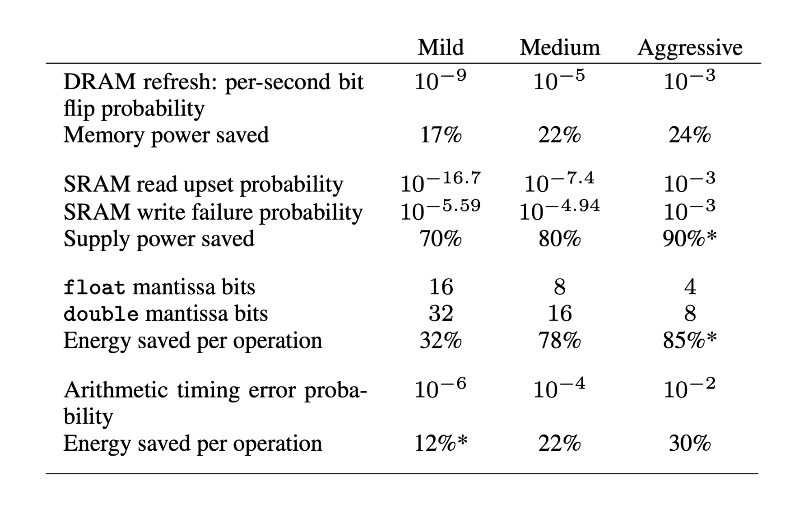
\includegraphics[scale=0.4]{enerj_hardware_model.png}
\end{center}

\subsubsection{Esperimenti}
Gli autori di EnerJ lo hanno testato su diversi programmi (con una percentuale di annotazioni fatte tra il $4\%$ e il $34\%$) ottenendo una riduzione del consumo dal $10\%$ al $50\%$ sopratutto nel passaggio dal programma base ad un approccio di annotazione \textit{mild}, con un aumento di un errore in questo caso sotto al $10\%$ e a volte anche prossimo allo $0\%$.